\chapter{Implementação}
\label{chap:impl}

Neste capítulo discutiremos tópicos relacionados à implementação do sistema de diarização de locutor proposto. 

Na seção \ref{sec:tools} apresentamos as ferramentas principais utilizadas no desenvolvimento deste trabalho.
Em seguida, na seção \ref{sec:preproc}, apresentamos o trabalho realizado para preparação e pré-processamento dos dados.

Foram desenvolvidos dois conjuntos scripts distintos para este trabalho; um sistema para treinamento da rede neural convolucional, e outro para a diarização de locutor em um vídeo com as características definidas anteriormente.
Sendo assim, discutiremos a arquitetura utilizada para treinamento do modelo na seção \ref{sec:train}, e a utilizada no processamento de uma mídia de entrada na seção \ref{sec:application}.

\section{Ferramentas}
\label{sec:tools}

Nesta seção apresentamos as principais ferramentas utilizadas durante a implementação deste trabalho.
Definiremos suas principais características, assim como as funcionalidades das mesmas que foram utilizadas, e as motivações por trás de sua escolha.

Na seção \ref{subsec:dlib} apresentaremos a biblioteca Dlib, utilizada para propósito de identificação e demarcação facial no projeto.
Em seguida, na seção \ref{subsec:tf} apresentaremos a biblioteca Tensorflow, utilizada por sua robusta implementação do modelo de rede neural convolucional.
Na seção \ref{subsec:environ} apresentaremos o ambiente utilizado para treinamento do modelo, assim como seus recursos computacionais.
Por fim, na seção \ref{subsec:otools}, mencionaremos brevemente as demais ferramentas utilizadas em caráter pontual no trabalho, e que, por essa razão, não receberam seções dedicadas.

\subsection{Dlib}
\label{subsec:dlib}
A Dlib\cite{dlib09} é uma biblioteca de código aberto desenvolvida em C++ e com interface em Python.
Trata-se de uma biblioteca generalista, contendo implementações de algoritmos para processamento paralelo, grafos, entre outros.
Porém, seu foco principal se encontra nas áreas de aprendizado de máquina, processamento de imagem e reconhecimento facial.

A biblioteca possui um identificador facial baseado em \textit{Histogram of Oriented Gradients} (HOG) capaz de detectar rostos frontais mesmo em imagens de baixa resolução.
As características específicas deste reconhecedor foram discutidas na seção \ref{sec:faciallm}.

% FIXME: Colocar mais aprofundadamente na fundamentação teórica
% HOG é uma técnica de visão computacional na qual são calculados gradientes para cada pixel da imagem a partir de seus vizinhos de forma a identificar as fronteiras entre os objetos da figura. Os gradientes calculados são então utilizados para computar blocos descritores de 8x8 pixels com 9 canais. Esses blocos sofrem normalização local para compensar fatores como a iluminação do ambiente, e servem como entrada para uma Máquina de Vetores de Suporte, resultando em um reconhecedor de faces rápido e robusto. Uma explicação mais aprofundada sobre esta técnica pode ser obtida em \cite{dalalHistogramsOrientedGradients2005}.

\begin{figure}[ht]
    \centering
    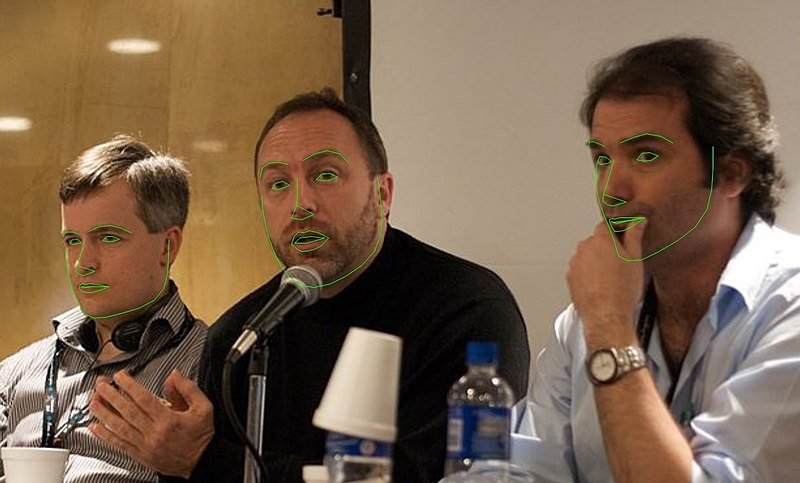
\includegraphics[width=0.7\textwidth]{dlib-face_landmark_detection.jpg}    
    \caption{Detecção de Marcadores Faciais pela biblioteca Dlib. Imagem publicada sob licença Creative Commons\cite{mtheilerDeteccaoMarcadoresFaciais2019}. }
    \label{fig:dlib-landmarking}
\end{figure}

Além disso, a mesma implementa um detector de marcadores faciais baseado em uma floresta de árvores de regressão, capaz de identificar (ou estimar, caso não estejam visíveis) as posições de um conjunto de pontos em um rosto, como mostra a figura \ref{fig:dlib-landmarking}.
A biblioteca fornece também um modelo pré-treinado para este detector para identificação de 68 destes marcadores, sob licença que permite uso acadêmico.
Esta funcionalidade foi chave para a escolha da biblioteca para a implementação do trabalho, visto que permitiu o treinamento do classificador utilizando um conjunto menor de dados, sem preocupações quanto a vieses relacionados às características físicas do locutor.

A biblioteca Dlib foi utilizada em sua versão 19.19.0, compilada a partir do código fonte com suporte para GPU e otimizações referentes à arquitetura da CPU.

\subsection{Tensorflow}
\label{subsec:tf}

Tensorflow\cite{tensorflow2015-whitepaper} é um framework de código aberto para aplicações de aprendizado de máquina.
A biblioteca, construída pela empresa Google, apresenta implementações robustas de diversos algoritmos da área, além de uma API que permite a declaração de uma rede neural em função de suas camadas.
A biblioteca suporta, ainda, o uso de uma ou mais GPUs para treinamento da rede neural, através da biblioteca cuDNN. No trabalho, essa foi utilizada para assistir na modelagem da rede neural, assim como seu treinamento e posterior execução como parte do sistema completo.

A escolha desta biblioteca se deu devido à sua implementação de algoritmos chave para o desenvolvimento do trabalho, tais como a rede neural convolucional tridimensional, discutida na seção \ref{sec:ann}.
Além disso, suas interfaces nas linguagens de programação C++ e Python, assim como a facilidade de utilização de interface em Python para prototipagem rápida de redes neurais convolucionais com topologias diferentes foram decisivas para sua escolha para a realização do trabalho.

Nesse trabalho, utilizamos a versão do Tensorflow 2.1.0, compilada a partir do código fonte com suporte para GPU e otimizações do referentes à arquitetura da CPU.

\subsection{Ambiente de Desenvolvimento}
\label{subsec:environ}

No desenvolvimento deste trabalho foi utilizada em caráter primário a linguagem de programação Python.
Originalmente, o trabalho seria desenvolvido em C++ devido ao mais alto desempenho desta linguagem; no entanto, a utilização de diversas bibliotecas com interface em Python assim como o mais rápido desenvolvimento e prototipagem nesta linguagem levou à decisão final de utiliza-la para a implementação do projeto.

A IDE utilizada no desenvolvimento foi o Visual Studio Code, ferramenta de código aberto criada pela Microsoft, e o Jupyter Notebook\cite{kluyverJupyterNotebooksPublishing2016}, por sua capacidade de subdividir e visualizar o estado do programa em execução.
%O treinamento da rede neural foi realizado em máquina com sistema operacional Windows 10, equipada com uma CPU Intel Core i7 de quarta geração, 12 GB de memória RAM e uma GPU Nvidia GTX 980 com 4 GB de memória dedicada.
O treinamento da rede neural foi realizado em máquina com sistema operacional Ubuntu Linux 16.04, equipada com uma CPU Intel Core i7 de primeira geração, 12 GB de memória RAM, e uma GPU Nvidia GTX 1080 Ti com 12 GB de memória dedicada.

\subsection{Outras Ferramentas}
\label{subsec:otools}

Nesta seção apresentamos as demais bibliotecas utilizadas no desenvolvimento do projeto. Em cada subseção descrevemos brevemente a biblioteca, definindo seu papel no projeto.

As bibliotecas se encontram ordenadas por sua função na pipeline do classificador, discutida de forma mais aprofundada na seção \ref{sec:train}.

\subsubsection{OpenCV}

OpenCV\cite{opencv_library} é uma biblioteca de código aberto para aplicações de Visão Computacional.
Ela foi utilizada para realizar a leitura quadro a quadro dos arquivos de vídeo a serem processados pelo sistema, e para codificar em vídeo a saída do classificador.
Neste trabalho foi utilizada a biblioteca opencv-python em sua versão 4.2.0.32.

\subsubsection{Matplotlib}

A Matplotlib\cite{hunterMatplotlib2DGraphics2007} é uma biblioteca para produção de gráficos e imagens em Python.
Ela foi utilizada para produzir as imagens intermediárias, através do desenho de polígonos a partir dos vértices produzidos pelo processo de detecção de marcadores facial.
Neste trabalho utilizamos a Matplotlib na versão 3.1.3 da biblioteca.

\subsubsection{Pandas}

Pandas\cite{mckinney-proc-scipy-2010} é uma biblioteca de processamento de dados em Python.
Ela foi utilizada no pré-processamento dos dados com a finalidade de manipular os arquivos csv contendo a diarização manual dos vídeos do dataset de depoimentos.
A biblioteca foi utilizada em sua versão 1.0.0.

\subsubsection{Scikit Learn e dscore}

As bibliotecas Scikit-Learn\cite{pedregosaScikitlearnMachineLearning2011}, biblioteca de aprendizado de máquina tradicional em python, e dscore\cite{ryantNryantDscore2020}, biblioteca para cálculo de métricas de diarização, foram utilizadas para o cálculo de diversas métricas relacionadas ao desempenho do sistema.
Essas foram utilizadas em suas versões 0.22.2.post1 e 1.1.0, respectivamente.

\section{Preparação dos Dados}
\label{sec:preproc}

Originalmente, foi fornecido pela Defensoria Pública do Estado do Rio de Janeiro um dataset contendo 29 vídeos, totalizando cerca de 5 horas de vídeo, referente a depoimentos prestados por diferentes participantes.
Os vídeos fornecidos apresentam resolução de $320\times240$ pixels, a uma taxa de 30 quadros por segundo.
O conjunto de dados não apresentava nenhuma anotação referente à fala dos depoentes.

Primeiramente, segmentamos os vídeos em fragmentos de 15 quadros, ou meio segundo.
A motivação para a segmentação do vídeo de entrada em trechos deste comprimento foi a estipulação de que o tempo necessário para a fala da primeira sílaba em uma frase, por uma pessoa normal, no português do Brasil, é de 252 milissegundos\cite{barbosaSyllabletimingBrazilianPortuguese2000}.
Sendo assim, ao dobrar este tempo, adquirimos a capacidade de detectar por completo o movimento do locutor quando referente a frases curtas, tais como interjeições.

Estes trechos foram validados para determinar se a face do depoente poderia ser reconhecida, com finalidade de descartar fragmentos nos quais este não olhava em direção à câmera, ou nas quais o detector HOG não poderia identifica-los.
Cada trecho foi então manualmente classificado quanto à ocorrência de fala pelo depoente, produzindo uma tabela que associava o identificador de cada arquivo à classe correspondente ao mesmo.

Feita essa diarização manual, os vídeos foram separados em conjuntos de teste e treinamento, tais que vídeos diferentes seriam utilizados para cada fase do treinamento da rede neural.
Fizemos essa separação pois, como os fragmentos possuem relação temporal tanto entre si quanto com outros vídeos do mesmo depoente, seria possível que o treinamento da rede neural utilizando segmentos semelhantes aos fragmentos de teste pudesse inflar artificialmente o desempenho da mesma.

%Por fim, as diarizações produzidas manualmente foram utilizadas para organizar os fragmentos em uma estrutura de diretórios, tal que primeiramente estivessem separados por conjunto de teste ou treinamento, depois por vídeo de origem, e por fim por classe.
%Essa estrutura foi construída de tal forma que as informações relevantes ao gerador de amostras da rede neural pudessem ser obtidas todas a partir do caminho para o mesmo no sistema de arquivos.

Para a execução de todas essas tarefas foram desenvolvidos scripts em Python e Bash, capazes de segmentar os vídeos do dataset e de validar, mover, e organizar os fragmentos extraídos destes.
O código referente a estes pode ser encontrado no apêndice \ref{apdx:src}.

\section{Treinamento}
\label{sec:train}

Para o treinamento do modelo foi desenvolvido um sistema composto por dois componentes principais.

\begin{figure}[ht]
    \centering
    \fontsize{10pt}{10pt}\selectfont
    \includesvg[width=0.85\textwidth]{architecture.svg}
    \caption{A sequência de carregamento dos dados e treinamento do modelo.}
    \label{fig:arch_train}
\end{figure}

Primeiramente, foi construído um gerados de dados com a finalidade de alimentar os dados da entrada ao modelo dinamicamente. As características e funcionalidades se encontram descritas na seção \ref{sec:data-gen}.
Depois, foi definida a topologia do modelo de rede neural, discutida na seção \ref{sec:topology}, e os critérios e parâmetros relevantes ao fluxo de treinamento, discutidos na seção \ref{sec:train-flow}.

\subsection{Gerador de Dados}
\label{sec:data-gen}
A função primária do gerador de dados é carregar dinamicamente os vídeos a serem alimentados ao modelo em cada etapa de seu treinamento.
Um módulo capaz de realizar tal carregamento dinâmico foi necessário devido ao grande volume de dados sendo processados, por virtude de se tratarem de dados de vídeo.
Para isto, ele é inicializado com uma lista dos arquivos a serem carregados, assim como uma série de parâmetros que definem aspectos de sua operação, tais como o tamanho da batelada ou o pré-processamento a ser aplicado aos quadros.

Cada vídeo fornecido ao gerador é, ainda, invertido horizontalmente.
Isso é feito para garantir que o modelo fosse treinado para funcionar independentemente do ângulo do rosto do sujeito, desde que reconhecível pelo HOG, visto que na grande maioria dos vídeos do dataset original o falante se encontrava olhando para o lado esquerdo da câmera ou diretamente para esta.

Para acelerar o processo de identificação facial e detecção de marcadores faciais, o gerador é, ainda, capaz de processar múltiplos fragmentos em paralelo na CPU, além de manter um cache dos fragmentos processados em iterações anteriores do treinamento.
O paralelismo possibilitou a redução do tempo de execução da primeira iteração do treinamento e teste de cerca de 9 horas para aproximadamente uma hora e quarenta minutos, uma redução de 80\% no tempo de execução, enquanto a implementação do cache reduziu o tempo necessário para etapas subsequentes do processo de para cerca de 3 minutos.

\subsection{Pré-Processamento}
\label{sec:pre-processing}

\begin{figure}[ht]
    \centering
    \includesvg[width=1\textwidth]{loader_rgb.svg}
    \includesvg[width=1\textwidth]{loader_gray.svg}
    \includesvg[width=1\textwidth]{loader_lm.svg}
    \caption{A saída do gerador de dados em cada um de seus três modos de operação.}
    \label{fig:generator_out}
\end{figure}

O gerador de dados possui 3 modos distintos de operação, que correspondem aos filtros de pré-processamento que podem ser aplicados aos quadros carregados para compor a entrada do modelo de predição. Estes são:

\begin{itemize}
    \item RGB: Nesse modo, o quadro é codificado em padrão RGB, ou seja, com cores representadas por suas componentes vermelha, verde, e azul, nessa ordem.
    \item Grayscale: Nesse modo, o quadro RGB é convertido para escala de cinza, segundo a função $Y = 0.299 R + 0.587 G + 0.114 B$.
    \item Landmarks: Nesse modo, é gerada uma imagem em preto e branco, rasterizada a partir dos pontos identificados pela detecção de marcadores faciais em cada quadro carregado. Este foi o modo utilizado na implementação final do trabalho.
\end{itemize}

Em nossa implementação final, utilizamos o modo de \textit{landmarks}. Esse modo de operação implementa o seguinte algoritmo:

\begin{enumerate}
    \item O segmento de vídeo é carregado do disco quadro a quadro. 
    \item Os quadros passam por um identificador facial, que retorna coordenadas de retângulos que contêm rostos no quadro original.
    \item Os rostos identificados passam por um detector de marcadores faciais, que retorna o conjunto de 68 pontos correspondentes a seus marcadores.
    \item Os pontos são utilizados para o desenho de polígonos representativos do rosto sobre um canvas branco de mesmo tamanho da imagem original, na etapa à qual nos referimos como rasterização.
    \item A imagem rasterizada é recortada segundo o retângulo delimitado pelo identificador facial e alinhada horizontalmente.
\end{enumerate}

\subsection{Topologia do Modelo}
\label{sec:topology}

Para o modelo de predição, definimos uma topologia baseada na arquitetura VGG\footnote{VGG é uma arquitetura para redes neurais convolucionais para reconhecimento de objetos em fotos, desenvolvida pelo Grupo de Geometria Visual (do inglês Visual Geometry Group) da universidade de Oxford \cite{simonyanVeryDeepConvolutional2015}.}, que consiste em um número de pares de camadas de convolução e \textit{max pooling}, seguidas de camadas densamente conectadas.
A arquitetura foi adaptada para lidar com dados de caráter tri-dimensional.

\begin{figure}[ht]
    \centering
    \resizebox{!}{0.7\textheight}{
        \newcommand{\GenericLayer}[5]{
    \begin{minipage}{0.3\textwidth}
        \centering
        \baselineskip=1.25\baselineskip
            {\footnotesize{#2} \hfill \footnotesize{#3} \hfill \footnotesize{#4}}%
            \linebreak
            {\textbf{#1}}%
            \linebreak
            {\small{#5}}
    \end{minipage}%
}
\newcommand{\BasicLayer}[2]{
    \begin{minipage}{0.3\textwidth}
        \centering
        \baselineskip=1.25\baselineskip
            {\textbf{#1}}%
            \linebreak
            {\small{#2}}
    \end{minipage}%
}
\newcommand{\ConvLayer}[4]{
    \GenericLayer{#1}{K: (#2)}{}{\textbf{F: #3}}{#4}%
}
\newcommand{\PoolLayer}[3]{
    \GenericLayer{#1}{S: #2}{}{}{#3}%
}
\newcommand{\DenseLayer}[2]{
    \BasicLayer{#1}{S: #2}%
}
\newcommand{\InputLayer}[2]{
    \BasicLayer{#1}{#2}%
}

\begin{tikzpicture}[]
    \node[state, rectangle, align=center, fill=blue!20!white] (input) [] {
        \InputLayer{Entrada}{$15\times150\times150$}%
    };
    \node[state, rectangle, align=center] (conv3d_1) [below=of input] {
        \ConvLayer{Convolução 3D}{$4\times3\times3$}{16}{$12\times148\times148$}%
    };
    \node[state, rectangle, align=center] (maxpool_1) [below=of conv3d_1] {
        \PoolLayer{Max Pooling 3D}{$(2\times2\times2)$}{$6\times74\times74$}%
    };
    \node[state, rectangle, align=center] (conv3d_2) [below=of maxpool_1] {
        \ConvLayer{Convolução 3D}{$3\times3\times3$}{32}{$4\times72\times72$}%
    };
    \node[state, rectangle, align=center] (maxpool_2) [below=of conv3d_2] {
        \PoolLayer{Max Pooling 3D}{$(2\times2\times2)$}{$2\times36\times36$}%
    };
    \node[state, rectangle, align=center] (conv3d_3) [below=of maxpool_2] {
        \ConvLayer{Convolução 3D}{$1\times3\times3$}{64}{$2\times34\times34$}%
    };
    \node[state, rectangle, align=center] (maxpool_3) [below=of conv3d_3] {
        \PoolLayer{Max Pooling 3D}{$(2\times2\times2)$}{$1\times17\times17$}%
    };
    \node[state, rectangle, align=center] (dense_1) [below=of maxpool_3] {
        \DenseLayer{Densa}{$256$}%
    };
    \node[state, rectangle, align=center] (dense_2) [below=of dense_1] {
        \DenseLayer{Densa}{$128$}%
    };
    \node[state, rectangle, align=center, fill=green!20!white] (sofmax) [below=of dense_2] {
        \DenseLayer{Softmax}{$2$}%
    };
    
    \draw[-{Latex[length=2mm]}] (input) -- (conv3d_1);
    \draw[-{Latex[length=2mm]}] (conv3d_1) -- (maxpool_1);
    \draw[-{Latex[length=2mm]}] (maxpool_1) -- (conv3d_2);
    \draw[-{Latex[length=2mm]}] (conv3d_2) -- (maxpool_2);
    \draw[-{Latex[length=2mm]}] (maxpool_2) -- (conv3d_3);
    \draw[-{Latex[length=2mm]}] (conv3d_3) -- (maxpool_3);
    \draw[-{Latex[length=2mm]}] (maxpool_3) -- (dense_1);
    \draw[-{Latex[length=2mm]}] (dense_1) -- (dense_2);
    \draw[-{Latex[length=2mm]}] (dense_2) -- (sofmax);
    
    \node[state, rectangle, yshift=-1.1cm, fill=red!20!white] (dropout_1) [right=of input] {
        \DenseLayer{Dropout Espacial}{$40\%$}%
    };
    \node[state, rectangle, yshift=-1.5cm, fill=red!20!white] (dropout_2) [right=of maxpool_2] {
        \DenseLayer{Dropout Espacial}{$35\%$}%
    };
    \node[state, rectangle, yshift=-1.5cm, fill=red!20!white] (dropout_3) [right=of maxpool_3] {
        \DenseLayer{Dropout}{$50\%$}%
    };
    \node[state, rectangle, yshift=-1.1cm, fill=red!20!white] (dropout_4) [right=of dense_1] {
        \DenseLayer{Dropout}{$25\%$}%
    };
    
    \draw[-{Latex[length=2mm]}] (dropout_1) |- (conv3d_1);
    \draw[-{Latex[length=2mm]}] (dropout_1) |- (conv3d_2);
    \draw[-{Latex[length=2mm]}] (dropout_2) |- (conv3d_3);
    
    \draw[-{Latex[length=2mm]}] (dropout_3) |- (dense_1);
    \draw[-{Latex[length=2mm]}] (dropout_4) |- (dense_2);
    
    \node[draw=none, fill=none, minimum size=0.3\textwidth] [left=of input] (placeholder) {};
\end{tikzpicture}
        }
    \caption{Topologia do Modelo}
    \label{fig:topology_typeA}
\end{figure}

\subsection{Treinamento do Modelo}
\label{sec:train-flow}

Em cada época, o sistema de treinamento do modelo chama o gerador de dados de treinamento, que lhe retorna um número fixo de amostras (batelada) compostas por segmentos de 15 quadros consecutivos.
O modelo então faz suas predições quanto a estas, e tem seus pesos ajustados através do algoritmo de retro-propagação de forma a minimizar uma função de custo.

\begin{equation} \label{eq:categorical_crossentropy}
    L(y,\hat{y})=-\sum\limits_{j=0}^M\sum\limits_{i=0}^N(y_{ij}*log(\hat{y}_{ij}))
\end{equation}

Como se trata de um problema de classificação, escolhemos como função custo do treinamento a função de entropia categórica cruzada, definida na equação \ref{eq:categorical_crossentropy}. Nessa equação, $\hat{y}$ é o vetor das probabilidades das categorias, e $y$ é a categoria real, codificada \textit{one-hot}\footnote{Codificação one-hot é o processo através do qual itens de um conjunto são codificados tal que sua representação seja uma sequência binária com um único bit ativo.}.

Visto que trata-se um problema de classificação binária, seria possível também utilizar a função de entropia cruzada binária; Porém, considerando a possibilidade de expansão futura do modelo para detecção de outras ações conversacionais, tais como gestos com a cabeça, decidimos utilizar uma função custo mais escalável para adição de novas classes.

Uma vez esgotadas as amostras de teste, o modelo chama, então, o gerador de dados de validação, realizando predições sem retro-propagação sobre as entradas retornadas, e calculando o valor da função custo para os resultados.
Esta etapa é fundamental para garantirmos que o modelo treinado seja aplicável a dados do mundo real, e não exclusivamente aos dados do conjunto de treinamento.

Por fim, ao se esgotarem também essas amostras, dá-se o final de uma época do treinamento, e os geradores tem suas listas de arquivos embaralhadas de forma a garantir aleatoriedade na ordem da próxima época.
Ainda para prevenção de \textit{overfitting} na rede neural foi definido como critério de parada do treinamento a condição de que não haja redução da função custo durante cinquenta épocas do treinamento.

\section{Aplicação}
\label{sec:application}
